\StartPlate{V18}{The noncompact scalar obstruction survives compact agreement}{Changing the full character removes one obstruction, not the occurrence problem.}
\begin{center}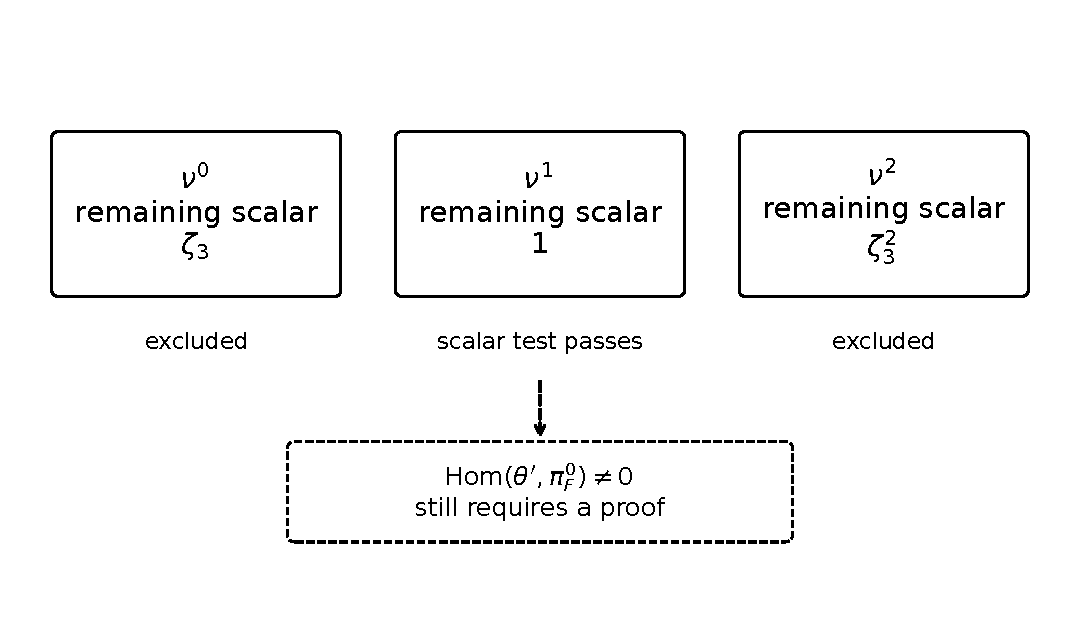
\includegraphics[width=\linewidth]{figures/V18.pdf}\end{center}
In continuation113, the original $\theta_0$ is compatible with the tested compact action but produces the wrong scalar at a noncompact generator. The retained intertwining and maximal-type arguments yield $\operatorname{Hom}_{H^1}(\theta_0,\pi_F^0)=0$ for the prescribed source-defined candidate.

The correction powers $\nu^a$, for $a=0,1,2$, leave generator scalars $\zeta_3,1,\zeta_3^2$. Only the middle correction passes this test. It changes the full character, rather than merely changing a basis. Its uniformizer value must also preserve the central normalization shown on V06.
\[
\operatorname{Hom}_{H^1}(\theta',\pi_F^0)\ne0
\quad\text{is still not established.}
\]
The new atlas recomputes the exact scalar exponents. It does not rerun the earlier local-field matrix programs or supply a new occurrence proof. Choosing some other representation that contains $\theta'$ would abandon the fixed-candidate question. Rescaling an intertwiner cannot remove a nontrivial scalar between two representations whose common compact restriction is irreducible.
\vfill\PlateSource{Inherited arithmetic obstruction with exact scalar model}{Part II, Section 18}{47}
